\chapter{KAGRA}
\section{Overview of KAGRA}
\subsection{Status of KAGRA}
KAGRA is a 3km laser interferometer constructed in Kamioka, Gifu, Japan, and is now in its final commisioning phase. KAGRA is now commisioning to observe with LIGO and Virgo in the third observation (O3), through the two test operation phase. The phases of KAGRA project is listed in Table \ref{tb:tb600}. The first test operation named initial KAGRA (iKAGRA), which is taken place from March to April 2016, was a demonstration of the 3-km Michelson interferometer. In this operation, While the test masses are not in cyogenic temperature but room temperature, KAGRA demonstrate the operation of the km-scale interferometer in the underground. Next, the second test operation named baseline KAGRA (bKAGRA) demonstrated the cryogenic Michelson interferometer from April to May 2018. Although this interferometer was not for sensitivity enhanced configuretion, the cryogenic operation, which is the key feature of KAGRA, could be demonstrated. Now, December 2019, KAGRA is faced on the O3 observation with the Michelson interferometer whose each arm have Fabry-Perot optical cavities (FPMI). To join the O3, KAGRA is now tunning the interferometer operation and hunting the sevelal technical noises.
\begin{table}[h]
  \caption{Summary of the phasec of KAGRA. MI: Michelson Interferometer, FPMI: Fabry-Perot Michelson Interferometer, DRFPMI: Dual-Recycled Fabry-Perot Michelson Interferometer, RSE: resonant sideband extraction}
  \begin{tabular}{lllll}
    \toprule
    &iKAGRA& \begin{tabular}{l}bKAGRA\\Phase1\end{tabular} & \begin{tabular}{l}bKAGRA\\for O3\end{tabular}  & \begin{tabular}{l}bKAGRA\\(final)\end{tabular}  \\ \midrule
        
        \begin{tabular}{l}Year\end{tabular}& \begin{tabular}{l}2016\\Mar - Apr\end{tabular}&\begin{tabular}{l}2018\\Apr - May\end{tabular} & \begin{tabular}{l}2019\\Dec - \end{tabular} & \begin{tabular}{l}2020 -\\(planned)\end{tabular} \\
              \begin{tabular}{l}Configuration\end{tabular} & \begin{tabular}{l}MI\end{tabular} & \begin{tabular}{l}MI\end{tabular} & \begin{tabular}{l}FPMI\end{tabular} & \begin{tabular}{l}DRFPMI\\(RSE)\end{tabular}\\
                      
                      \begin{tabular}{l}Test mass\\temperature\end{tabular} & \begin{tabular}{l}room temp.\end{tabular}& \begin{tabular}{l}18K\\room temp.\end{tabular} & \begin{tabular}{l}18K\\room temp.\end{tabular}  & \begin{tabular}{l}22K\end{tabular}             \\ \bottomrule
  \end{tabular}
\end{table}

%% KAGRAの最終的な感度は、resonant sideband extraction thechnique をもちいた Dual-Recycled Fabry-Perot Michelson interferometer で達成される。KAGRAの設計感度をFig.\ref{img:img600}に示す。

%% \begin{figure}[h]
%%   \begin{center}   
%%     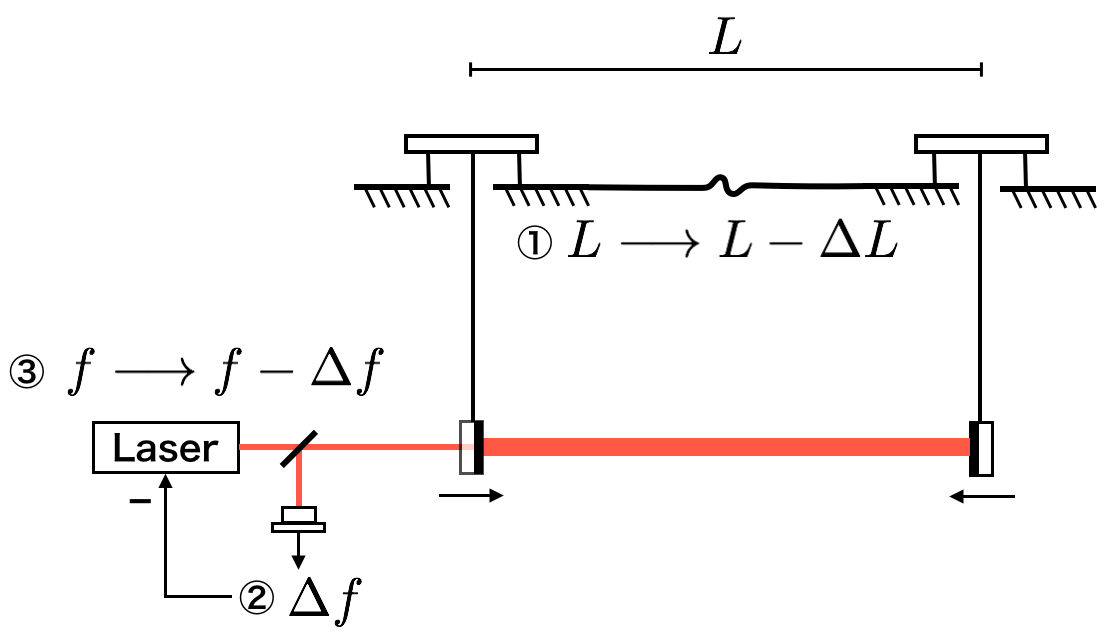
\includegraphics[width=12cm]{./img_chap6/img600.png}
%%     \caption{The designed sensitivity of KAAGRA \cite{akutsu2019first}}{}\label{img:img600}
%%   \end{center}
%% \end{figure}

\subsection{Main Interferometer}
The main interferometer of KAGRA is shown in Figure \ref{img:img601}. The interferometer configuration of KAGRA is also the same as other GW detectors such as advanced LIGO and advanced Virgo, the Michelson interferometer with Fabry-Perot optical cavity on each arm and two rycycling optical cavities. The different feature of these detectors is the cryogenic test masses. To cool down to cryogenic, tipicaly 22 K, the test mass mirror is made of sapphire because of the high thermal conductivity and mechanichal Q value even in cryogenic environment. These properties can reduce some problems of the interferometeric GW detectors; thermal lens effect and thermal noise.
\begin{figure}[p]
  \begin{minipage}{15cm}
    \begin{center}   
      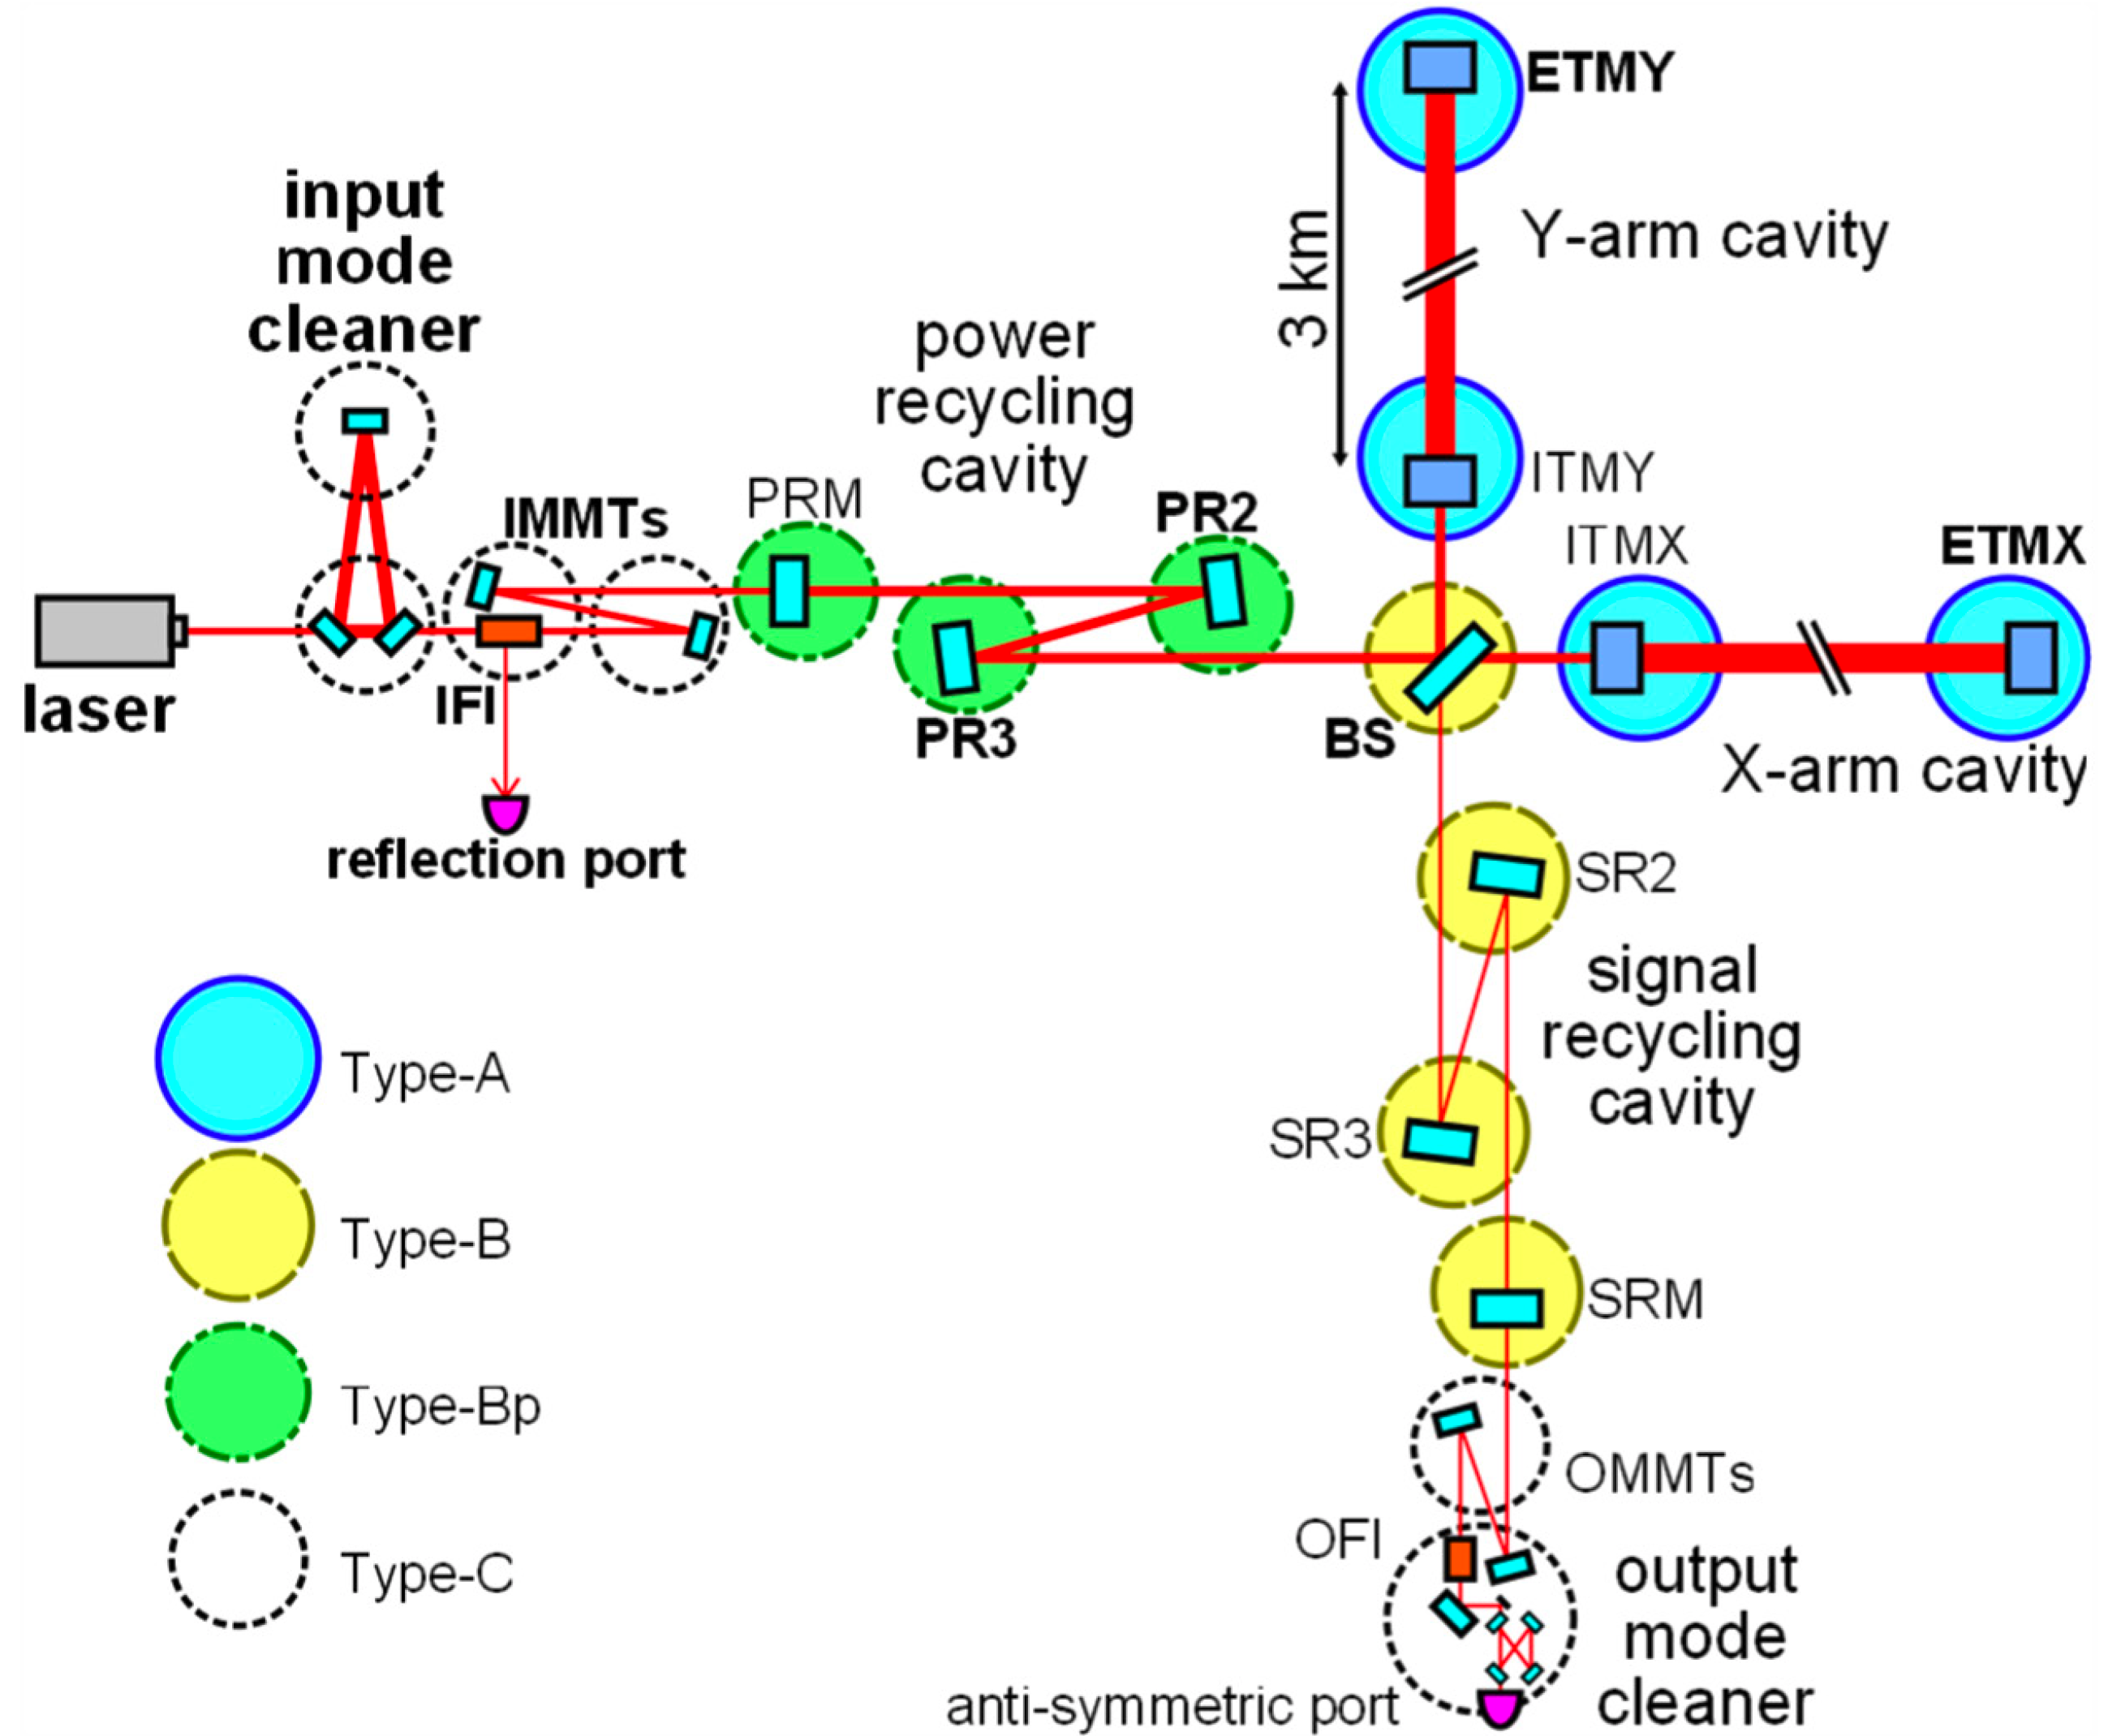
\includegraphics[width=13cm]{./img_chap6/img601.png}
      \subcaption{Schematic interferometer configuration of KAGRA \cite{akutsu2019first}}{}\label{img:img601} \hfill\vspace{10pt}
    \end{center}
  \end{minipage}
  \begin{minipage}{15cm}
    \begin{center}   
      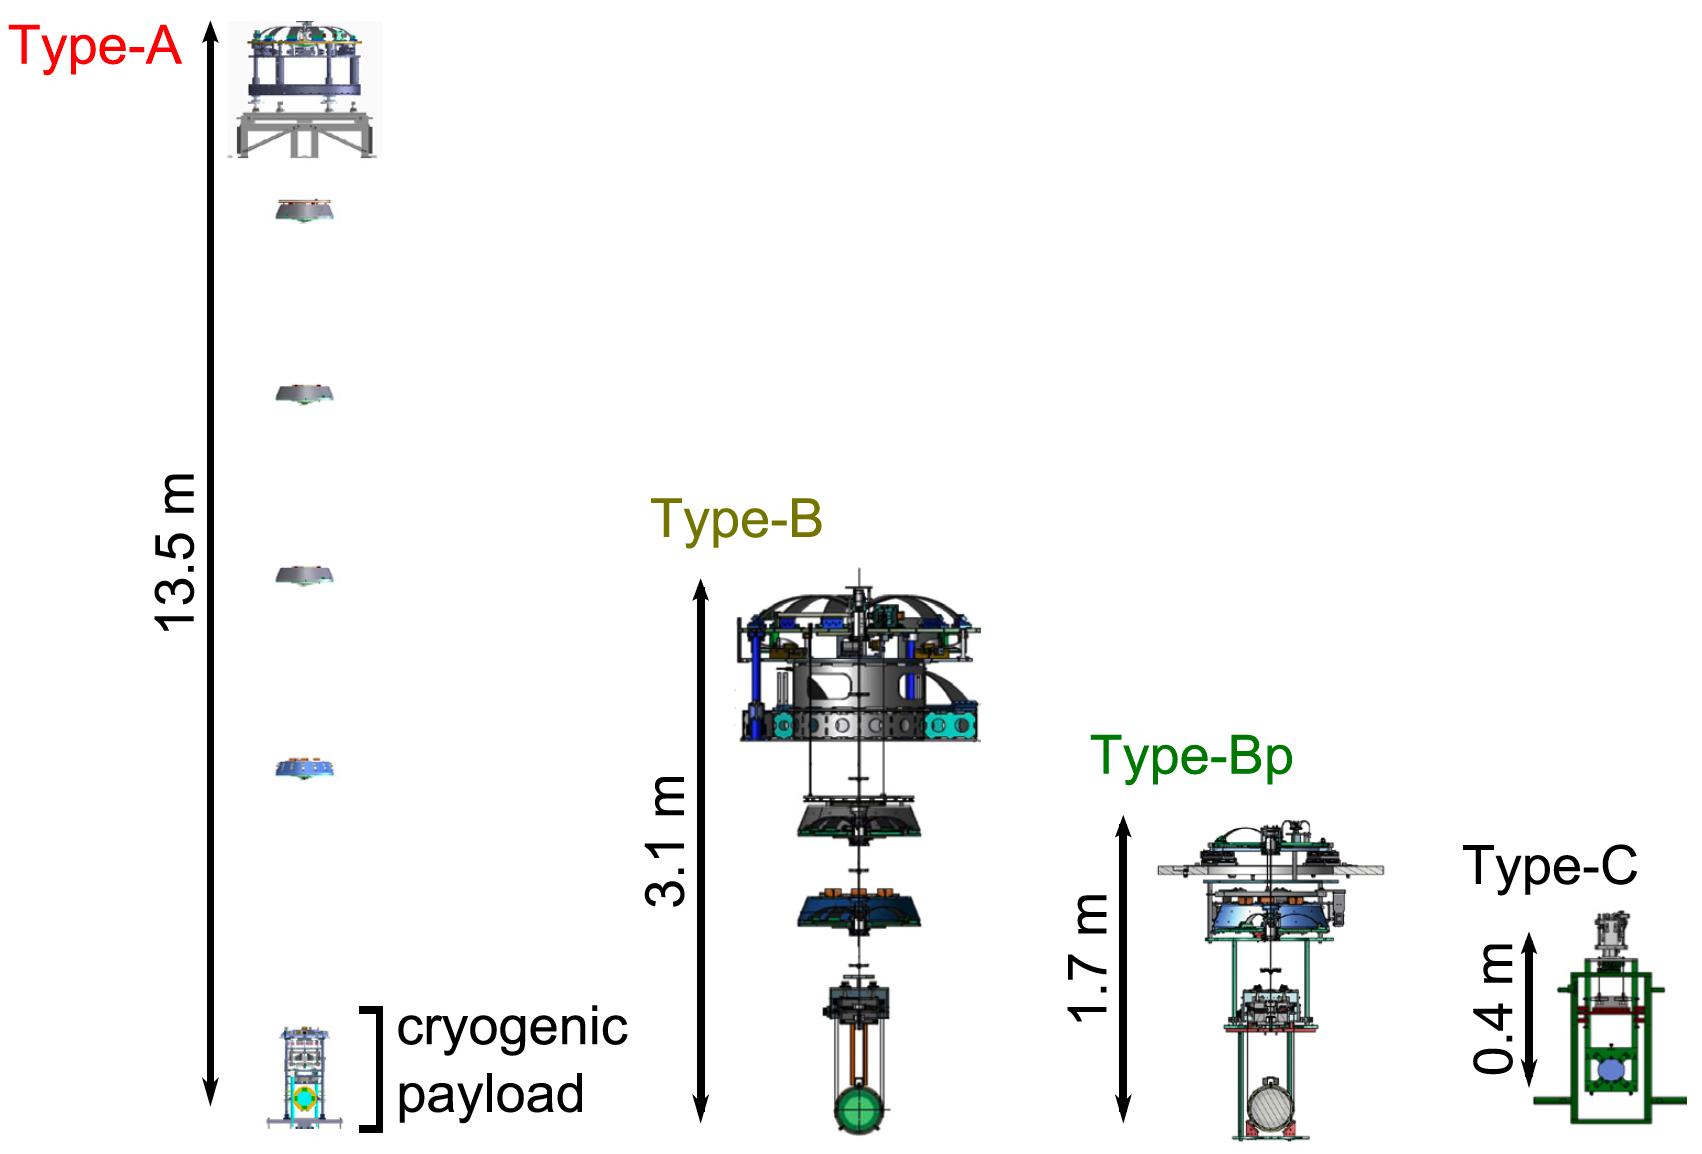
\includegraphics[width=13cm]{./img_chap6/img601b.png}
      \subcaption{KAGRA mirror suspension system \cite{akutsu2019first}}\label{img:img601b}
    \end{center}
  \end{minipage}
  \caption{Interferometer configuration and mirror suspension system}{}
\end{figure}
The main interferometer is divided into four parts; (1) arm caivties, (2) input and output mode cleaners (IMC and OMC), (3) power resycling cavities (PRC), (4) and signal resycling cavities (SRC). The first, the arm cavities are composed of input test masses (ITMs) and end test masses (ETMs) with high reflectivity corresponding to a finesse of 1530 not to increase the internal cavity power. The second, while IMC is used for clean out the higher-order spatial mode and stabilizing the frequency of main input laser, OMC is used for clean out the unwanted higher-order spatial modes and frequency sideband of the output beam. The IMC is the triangle optical cavity which is made to stabilize the input laser frequency above 1 Hz. The OMC is the bow-tie cavity composed of four mirrors. The third, PRC is used for increasing the input laser power by 10 times. This cavity is composed of three mirrors named PRM, PR2 and PR3, respectively. The forth, SRC is used for expand the bandwidth of GW signals.This technique is more important than Advanced LIGO and Advanced Virgo, because the bandwidth is narrower than other detectors due to a high finesse arm cavity of KAGRA. 

\subsection{Mirror Suspension System}
All mirrors of the interferometer are suspended by four types suspensions; Type-A, Type-B, Type-Bp, Type-C. These suspensions are shown in Figure \ref{img:img601b}. The Type-A is a 13.5 m scale 9-stage pendulum suspending the test mass mirror. The Type-B is a small size of Type-A suspension for suspending the signal recycling mirrors and beam splitter mirror. The Type-Bp is also small size of Type-B but without the pre-isolator stage, which is for the power recycling mirrors. The type-C is the simple 2-stage suspension used in TAMA300 but with minor modification.
\begin{figure}[p]
  \begin{center}   
    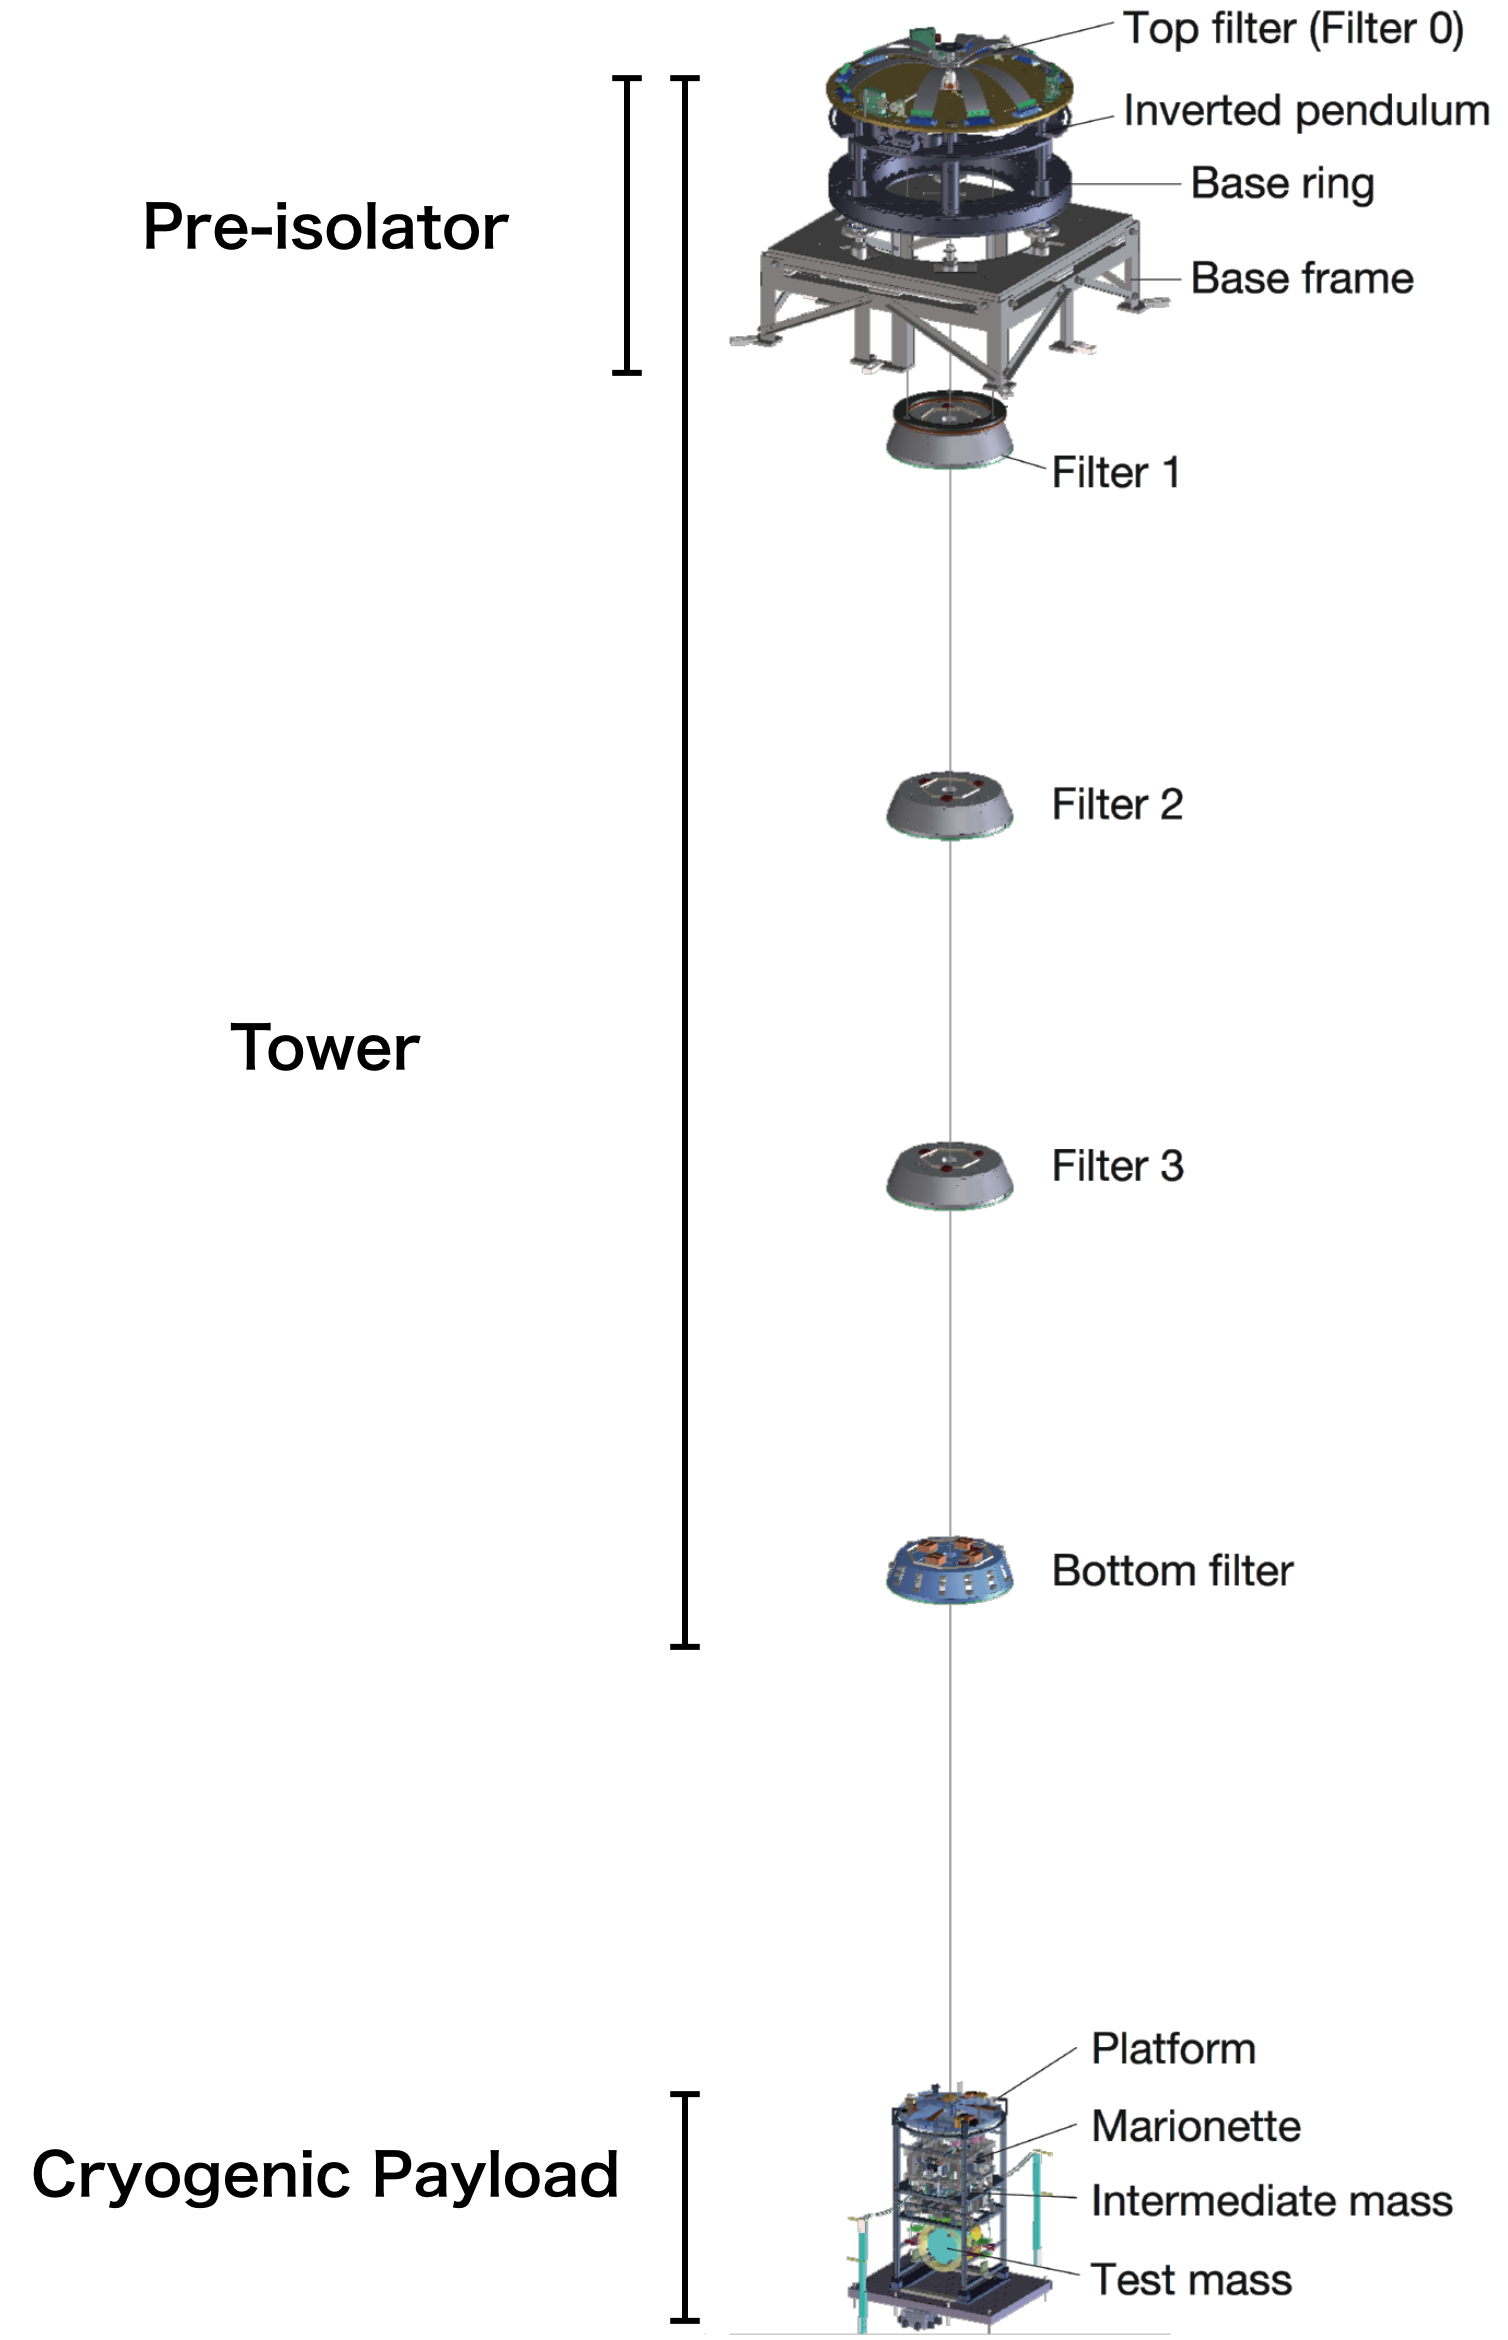
\includegraphics[width=13cm]{./img_chap6/img604.png}
    \caption{An overview of the Type-A suspension \cite{Okutomi2019development}. Test mass is suspend by a $13.5\,\mathrm{m}$ pendulum consisted of several mechanichal filters. The suspension point of the long pendulum is suported by the pre-isolator, which consists of inverted pendulum, on the ground through the base frame and base ring.}\label{img:img604}
  \end{center}
\end{figure}

\begin{figure}[p]
  \begin{minipage}{1.0\hsize}
    \begin{center}   
      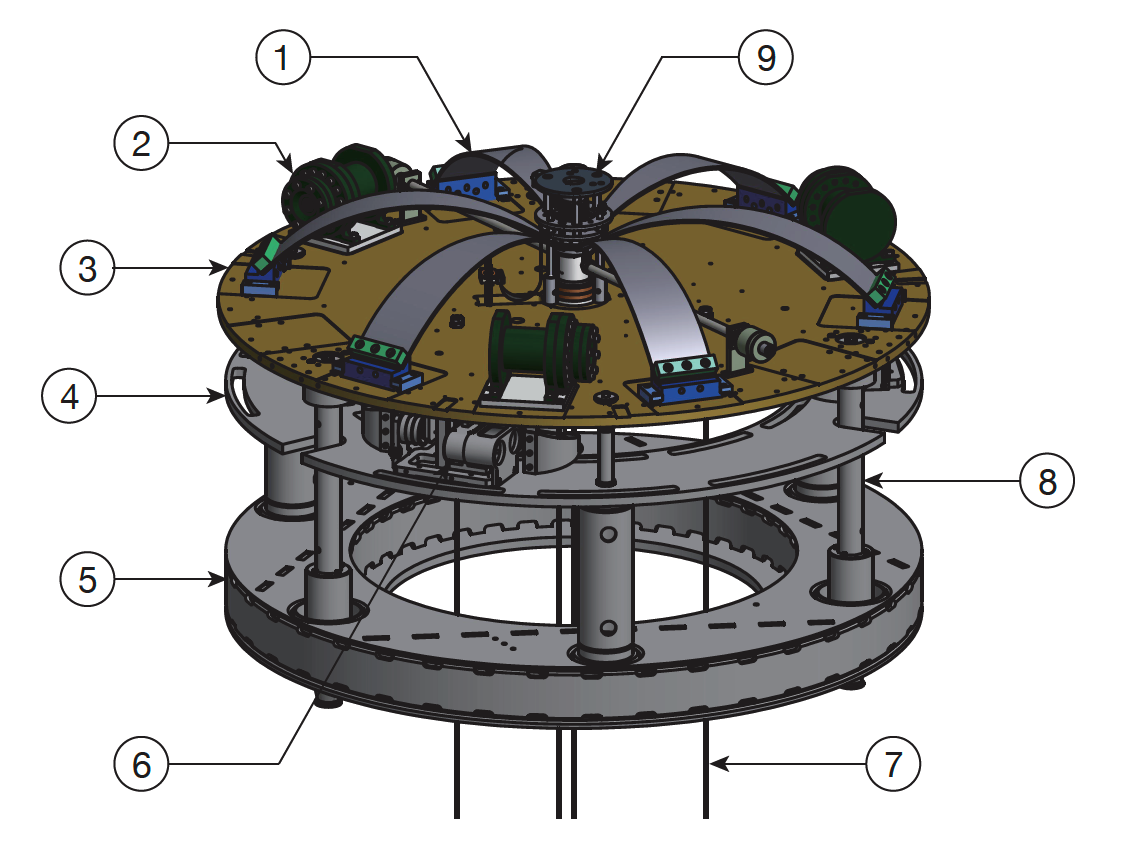
\includegraphics[width=12cm]{./img_chap6/img603a.png}
      \subcaption{Pre-isolator stage (PI). (1) Cantilever blade for GAS. (2) Geophone (3) Table of the top stage (4) Refernce frame rigidly connected to the base ring (5) The base ring mounted on the ground (6) LVDT and the coil magnet actuator (7) suspension wire to suspend the lower stages (8) leg of the inverted pendulum (IP). Figure is cited from figure 3.9 in \cite{Okutomi2019development}}\label{img:img603a}
    \end{center}
  \end{minipage}\\   
  \begin{minipage}[b]{0.5\hsize}
    \begin{center}
      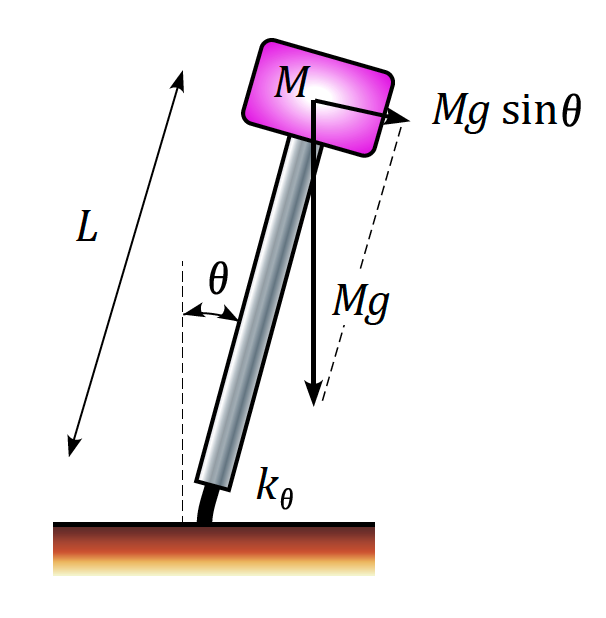
\includegraphics[width=8cm]{./img_chap6/img603b.png}
      \subcaption{Leg of the inverted pendulum (IP) \cite{sekiguchi2016astudy}.}\label{img:img603b}
    \end{center}
  \end{minipage}
  \begin{minipage}[b]{0.5\hsize}
    \begin{center}
      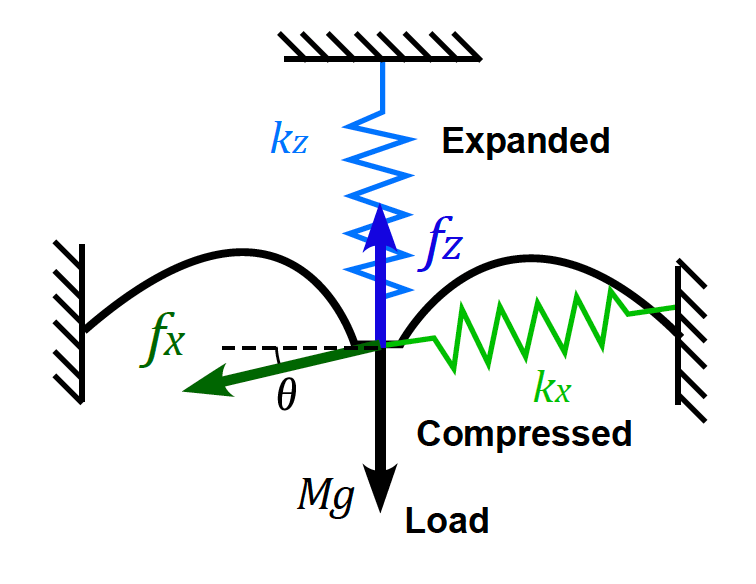
\includegraphics[width=8cm]{./img_chap6/img603c.png}
      \subcaption{Geometrical Anti-Spring \cite{sekiguchi2016astudy}.}\label{img:img603b}
    \end{center}
  \end{minipage}  
  \caption{CAD drawing of the pre-isolator (top) and main mechanical components of PI; IP leg and GAS (bottom).}
\end{figure}


\section{KAGRA Type-A Suspension}
\subsection{Overview}
In order to suspend the cryogenic test mass, as shown in Fig.\ref{img:img604}, KAGRA Type-A suspension has two parts; cryogenic payload and $13.5\,\mathrm{m}$ room temperature tower pendulum \cite{Okutomi2019development}. The cryogenic payload is consisted of Platform, Marionette, Intermediate mass, Test mass. The tower is consited of 5 mechanical filter; Top filter, F1, F2, F3, and Bottom filter. Moreover, the suspension point of tower is suspended by pre-isolator stage which has a inverted pendulum.

In terms of the low-frequency seismic attenuation, the pre-isolator is the important mechanical part.



\subsection{Pre-Isolator stage (PI)}
The pre-isolator (PI) is a active seismic iolator for the suspension point of the long Type-A or Type-B suspensions. As shown in Figure \ref{img:img603a}, the suspension point is on the platform stage suported by the inverted pendlum (IP) which isolates the seismic noise in horizontal direction. For vertical direction, geometric anti-spring (GAS) suspends this point. Especially, horizontal motion of the platform stage is isolated by using the feedback control with the inertial sensor and the relative position sensor, which is described in the section \cref{sec:512}.

\subsubsection{Inverted pendulum for horizontal vibration isolation}
Inverted pendulum (IP) is the low eigenfrequency pendulum because this mechanical filter can adjust the effective spring constant to small value by tuning the load on the platform stage. The angluar eigenfrequency of the singla IP leg is given by \cite{sekiguchi2016astudy}
\begin{eqnarray}
  \omega_{\mathrm{IP}}=\sqrt{\frac{g}{L}\left(\frac{k_{\mathrm{\theta}}/gL-M}{M}\right)},\\
\end{eqnarray}
where $k_{\theta}$ is the bending spring constant of the flexure, $M$ is the mass of the stage and $L$ is the length of the leg. Although the eigenfrequency ca be adjusted to zero in pronciple, actual eigenfrequency is designed at least 100 mHz because it is unstable when the term in square root is minus value.

\subsubsection{Geometric Anti-Spring for vertical vibration isolation}
Geometric anti-speing is also the low eigenfrequency pendlum in vertial direction. The eigenfrequency is adjusted to small value by compressing the cantilever blades as shown in Figure \ref{img:img603b}. The angular eigenfrequency is given by 
\begin{eqnarray}
  \omega_{\mathrm{GAS}} = \sqrt{\frac{1}{M}\left[{ k_{z}- \left(\frac{l_{0}}{x_{0}}-1\right) k_{x}}\right]},
\end{eqnarray}
where $M$ is the load mass, $k_{\mathrm{x}}$ and $k_{\mathrm{z}}$ are the elastic constant of the compressed catilevers, $l_{0}$ is a natural length of the blades, $x_0$ is the horizontal distance between the central keystone and the support poit of the blades. One can find that the angular eigenfrequency of the GAS is reduced when $x_{0}<l_{0}$.

\subsubsection{Liner Variable Differential Transducer (LVDT)}
\begin{figure}[h]
  \begin{center}   
    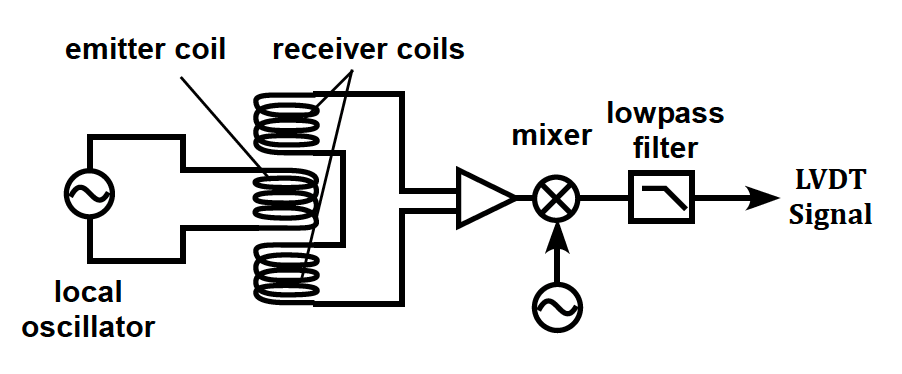
\includegraphics[width=10cm]{./img_chap6/img605.png}
    \caption{\cite{sekiguchi2016astudy}}\label{img:img605}
  \end{center}
\end{figure}
LVDT is a wide range relative position sensor composed of three coils \cite{Tariq2002hh}. shown in Fig.\ref{img:img605}. The emitter coil is mounted on the pre-isolator stage and driven with a sinusoidal signal to emit a modulated magnetic field. The two receiver coils is mounted on the reference structure, and these coils are counter-wound to each other. When the emitter coil is on the center of two reciever coils, induced voltage is not emitted from the reciever coils. On the other hand, when the pre-isolater is moved, a sinusoidal signal apprears on the reciever coils. Therefore, after demodulating this signal, amplitude of output signal is propotional to the displacement from the LVDT geometrical center.

\subsubsection{Coil-magnet actuator}
We use a voice-coil type wide range actuator to move the pre-isolator stage \cite{wang2002constant}.

